
%%%%%%%%%%%%%%%%%%%%%%%%%%%%%%

%% Produkt 2
%%%%%%%%%%%%%%%%%%%%%%%%%%%%%%
\begin{table}[!htbp] \centering	
	\label{fu:Temperatursensor1}
\begin{tabular}{|p{6cm}|p{8cm}|}
	\hline
		\textbf{Løsning}				&LM75, Digital temperatur sensor med two-wire interface. 			\\\hline %Produktnavn
		\textbf{Producent} 			&National semiconductors			\\\hline 
		\textbf{Tilslutning} 		&I2C 			\\\hline 
		\textbf{Beskrivelse} 		&Hardware modul der kan tilkobles enheden via I2C 			\\\hline 
		\textbf{Krav} 				&Indgående kendskab til I2C og PSoC creator 			\\\hline 
		\textbf{Fordele}			&Der er blevet lavet en øvelse i GFV, der omhandler denne type sensor. 			\\\hline 
		\textbf{Ulemper} 			&Den kommunikere over I2C som er mere besværligt at arbejde med. Der skal konstrueres en ''beholder'' til sensoren så den kan tåle at komme ned i jorden. 			\\\hline 
		\textbf{Pris} 				&Hentet fra værkstedet på IHA			\\\hline
		\textbf{Link} 				&\url{http://datasheets.maximintegrated.com/en/ds/LM75.pdf	}		\\\hline	
	
		\multicolumn{2}{|c|}
		{									%% Ændre filnavn uden endelse
		\raisebox{-0.91\height}{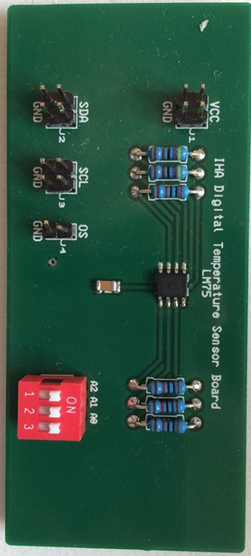
\includegraphics[height=3cm]{filer/forundersoegelse/billeder/LM75_temp_sensor}} 
		} \\\hline	

\end{tabular}
\end{table}
%%%%%%%%%%%%%%%%%%%%%%%%%%%%%%
\begin{table}[!htbp] \centering	
	\label{fu:Temperatursensor2}
\begin{tabular}{|p{6cm}|p{8cm}|}
	\hline
		\textbf{Løsning}				&DS18B20 temperatursensor. 			\\\hline %Produktnavn
		\textbf{Producent} 			&Dallas			\\\hline 
		\textbf{Tilslutning} 		&- 			\\\hline 
		\textbf{Beskrivelse} 		&Vandtæt temperaturprobe der kan tilkobles enhver microcontroller med en enkelt digital benforbindelse 			\\\hline 
		\textbf{Krav} 				&Indgående kendskab PSoC creator. 			\\\hline 
		\textbf{Fordele}			& Der er mulighed for at tilslutte flere af dem til den samme forbindelse, den kræver ingen ekstra HW. 			\\\hline 
		\textbf{Ulemper} 			&Dallas 1-Wire-protokollen  er lidt kompliceret, og kræver en del kode for at 											trække kommunikationen ud 			\\\hline 
		\textbf{Pris} 				&89 kr			\\\hline
		\textbf{Link} 				&\url{https://elextra.dk/main.aspx?page=article&artno=H15942	}		\\\hline		
	
	\multicolumn{2}{|c|}
		{									%% Ændre filnavn uden endelse
		\raisebox{-0.91\height}{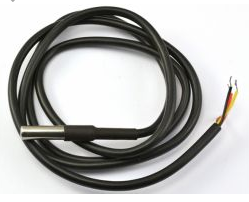
\includegraphics[height=3cm]{filer/forundersoegelse/billeder/Temp_sensor}} 
		} \\\hline	

\end{tabular}
\end{table}